\clearpage
\section{Results}

\subsection{Evaluation Methodology}

In this section, we evaluate the predictive capabilities of our learning models 
on unseen test data. The goal is to quantify how well each model generalizes to new inputs
and to compare their forecasting accuracy under the same experimental conditions. 
Such evaluation is crucial in financial forecasting tasks, where poor generalization 
can lead to significant mispredictions and financial loss.

To ensure a robust assessment, we compute four widely used regression metrics 
allowing for a detailed and balanced view of each model’s strengths and weaknesses. The  
following metrics will be used:

\begin{table}[H]
\centering
\caption{Evaluation Metrics for Stock Price Forecasting}
\label{tab:evaluation-metrics-usage}
\begin{tabular}{lp{3.5cm}p{3.5cm}p{4.5cm}}
\hline
\textbf{Metric} & \textbf{What It Measures} & \textbf{When It's Used} & \textbf{Why It Matters} \\
\hline\hline
\acrshort{rmse} &
  Square root of average squared differences between predicted and true values. &
  Used when large errors are more significant or costly. &
  Penalizes large deviations more strongly; useful for capturing general prediction accuracy. \\
\acrshort{mae} &
  Average absolute differences between predicted and actual values. &
  Useful when equal weight is given to all errors, regardless of size. &
  Easy to interpret and robust to outliers. Helps understand typical prediction error. \\
\acrshort{r2} &
  Proportion of variance in the target variable explained by the model. &
  Common in regression tasks to assess goodness of fit. &
  Indicates how well the model captures underlying data patterns (closer to 1 = better fit). \\
 \acrshort{mape} &
  Average absolute percentage difference between predicted and actual values. &
  Preferred when comparing model performance across different scales. &
  Scale-independent; expresses error as a percentage, making interpretation intuitive. \\
\hline
\end{tabular}
\end{table}

These metrics are widely adopted in stock price forecasting literature
\parencite{parmar2018stock, nabipour2020DeepLearning, agrawal2022StockPrediction, chang2024StockPrediction}
as they offer a comprehensive evaluation across error magnitude (\acrshort{rmse}, \acrshort{mae}), fit quality (\acrshort{r2}), and scale-independent accuracy (\acrshort{mape}).

Following the metric calculation, we interpret and compare the results, highlighting which 
model better captures temporal dependencies in stock price data. Special attention is 
given to overfitting behavior, model stability, and generalization performance. 

\subsection{Evaluation on Unseen Test Data}

In this section, we evaluate the performance of the final \acrshort{lstm} and \acrshort{lstmbigru} models
on the held-out test dataset, which was not seen during training or validation. This step assesses the 
model's generalization capabilities under realistic conditions and measures their ability to predict 
stock prices for completely new inputs.

Both models were used to generate next-day stock price predictions on the test set, and the outputs
were compared to the actual observed closing prices. The predictions were inverse-transformed using 
the original \texttt{MinMaxScaler} to return them to their real price scale.

These metrics allow a balanced assessment of performance by capturing average error, scale-normalized accuracy, and the proportion of explained variance. The results are summarized in Table~\ref{tab:test-metrics-comparison}.

\begin{table}[H]
\centering
\caption{Model Performance on Test Dataset}
\label{tab:test-metrics-comparison}
\begin{tabular}{lcccc}
\hline
\textbf{Model} & \textbf{RMSE} & \textbf{MAE} & \textbf{MAPE} & \textbf{R\textsuperscript{2}} \\
\hline\hline
LSTM & 5.1674 & 4.1259 & 4.88 & 0.9455 \\
LSTM-BiGRU & \textbf{1.9980} & \textbf{1.3178} & \textbf{1.27} & \textbf{0.9919} \\
\hline
\end{tabular}
\end{table}

The \acrshort{lstmbigru} model significantly outperformed the baseline \acrshort{lstm} model across all
metrics. Notably, it reduced the \acrshort{rmse} by more than half and achieved an \acrshort{r2} above 0.99, indicating that it explained nearly all the variance in the test data.

\subsection{Visual Comparison of Predictions}

Figure~\ref{fig:prediction-combined} shows the predicted stock prices over time for both models against the actual closing prices in the test set. This allows a visual inspection of how well each model tracks the true values and identifies deviations, lags, or systematic errors.

\begin{figure}[H]
    \centering
    \caption{Actual vs Prediction}
    \label{fig:prediction-combined}
    \begin{subfigure}[b]{\textwidth}
        \centering
        \caption{Actual vs Models}
        \label{fig:pred-full}
        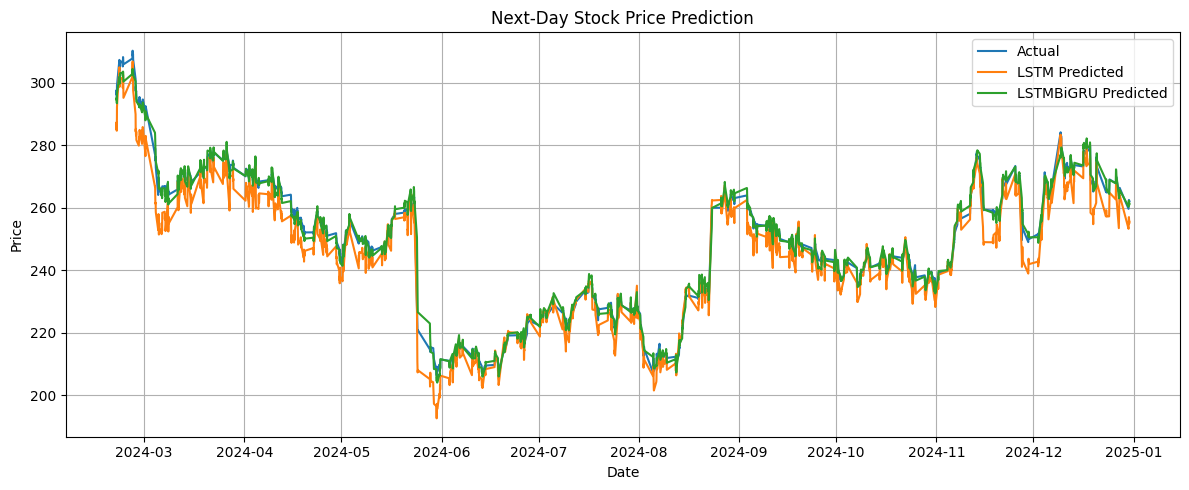
\includegraphics[width=\textwidth]{img/sections/main/pred-full.png}
    \end{subfigure}

    \vspace{0.5em}

    \begin{subfigure}[b]{0.48\textwidth}
        \centering
        \caption{Actual vs LSTM}
        \label{fig:pred-lstm}
        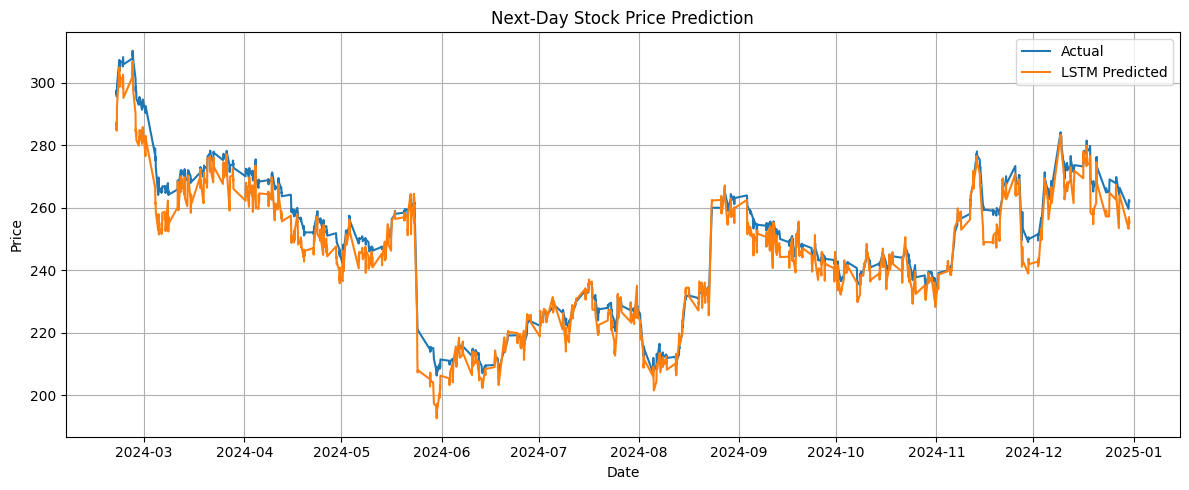
\includegraphics[width=\textwidth]{img/sections/main/pred-lstm.png}
    \end{subfigure}
    \hfill
    \begin{subfigure}[b]{0.48\textwidth}
        \centering
        \caption{Actual vs LSTM-BiGRU}
        \label{fig:pred-bigru}
        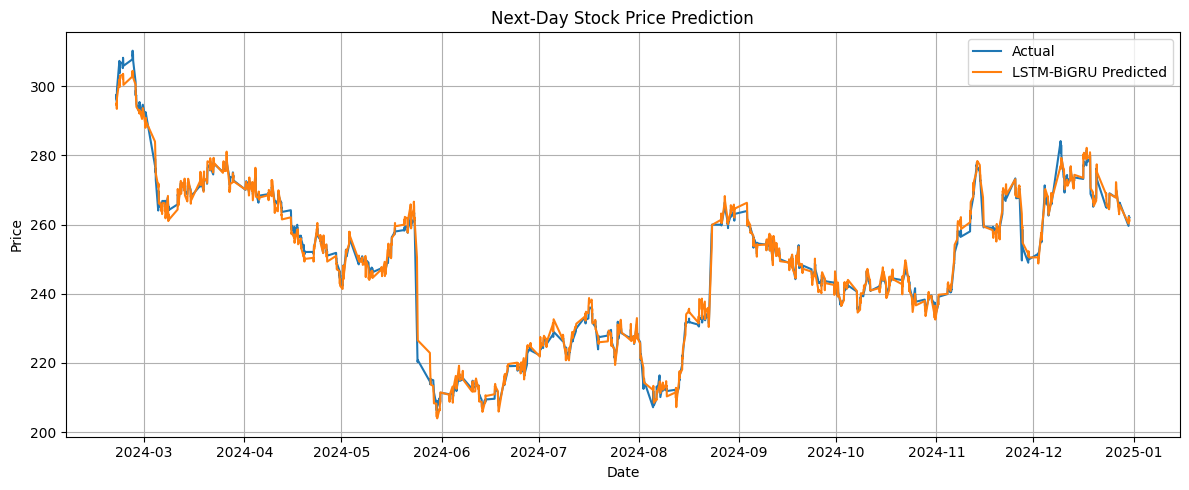
\includegraphics[width=\textwidth]{img/sections/main/pred-bigru.png}
    \end{subfigure}
\end{figure}

As shown in the figure, the \acrshort{lstmbigru} model exhibits tighter alignment 
with the real values, especially during volatile periods or sharp price changes 
(as an example we can look at End of February or End of May). This
suggests a better temporal understanding and generalization capacity. The standalone
LSTM model, while effective, displays slightly larger prediction deviations and 
smoothing during abrupt changes.

\subsubsection{Results Conclusion}

The comparison between predicted and actual values on the test set demonstrates that 
both the \acrshort{lstm} and the hybrid \acrshort{lstmbigru} models are capable of 
capturing temporal dependencies in stock price data, producing forecasts that follow 
real market trends closely. The error metrics indicate that these models generalize 
well to unseen data.

Among the two, the \acrshort{lstmbigru} model achieved superior performance across 
all metrics, aligning with recent research findings that hybrid deep learning 
architectures often enhance prediction accuracy for financial time 
series~\parencite{balasubramanian2023SystematicSurvey}. Based on 
Figure~\ref{fig:prediction-combined}
where the \acrshort{lstmbigru} model exhibits better alignment with sudden 
price shifts.

Importantly, this study extends prior research by evaluating model performance on 
\acrfull{wday}, a mid-cap stock characterized by high volatility and comparatively 
limited media and analyst coverage. Unlike large-cap stocks frequently used in 
previous studies, \acrshort{wday} presents a more realistic and challenging test case 
for financial forecasting models. The strong results from the \acrshort{lstmbigru} model 
in this context suggest that hybrid deep learning architectures not only scale to 
lower-information, high-volatility environments but may also provide valuable 
predictive improvements in such settings.
